%\documentclass{standalone}
%\usepackage{tikz}
%\usetikzlibrary{patterns,plotmarks}
%\begin{document}
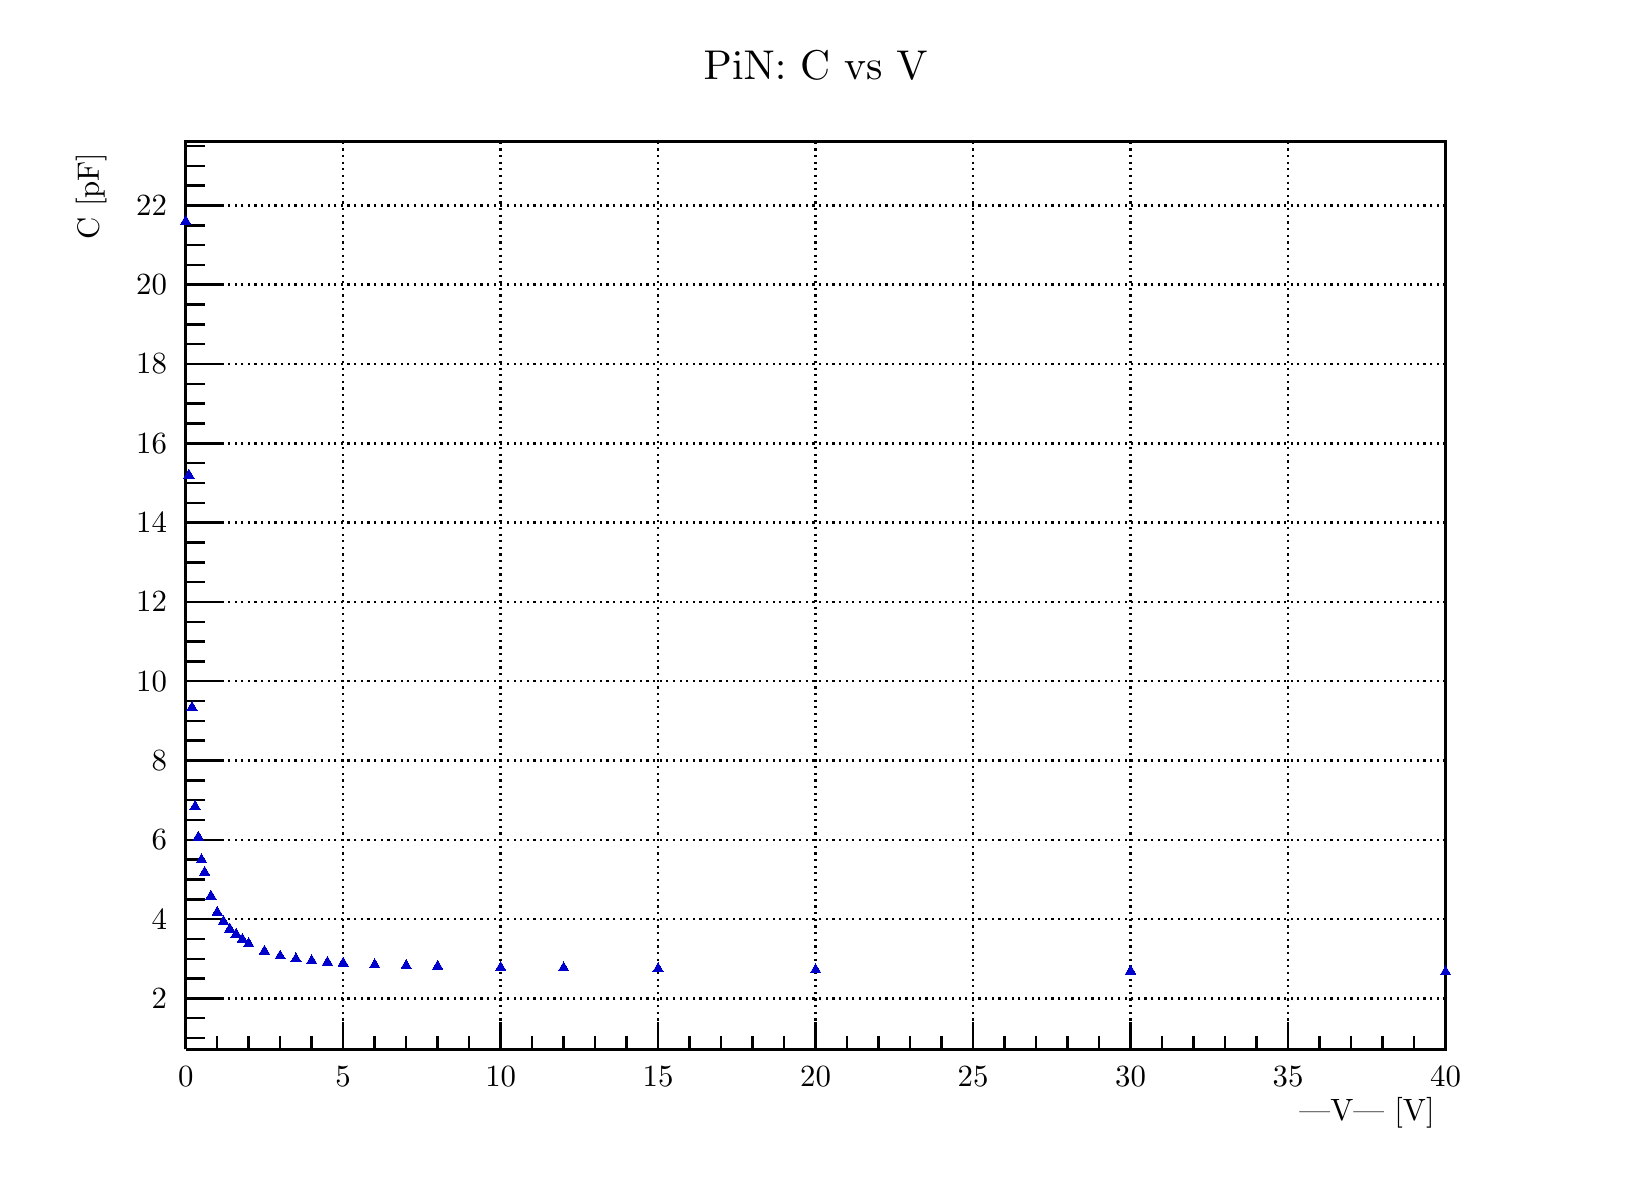
\begin{tikzpicture}
\def\CheckTikzLibraryLoaded#1{ \ifcsname tikz@library@#1@loaded\endcsname \else \PackageWarning{tikz}{usetikzlibrary{#1} is missing in the preamble.} \fi }
\CheckTikzLibraryLoaded{patterns}
\CheckTikzLibraryLoaded{plotmarks}
\pgfdeclareplotmark{cross} {
\pgfpathmoveto{\pgfpoint{-0.3\pgfplotmarksize}{\pgfplotmarksize}}
\pgfpathlineto{\pgfpoint{+0.3\pgfplotmarksize}{\pgfplotmarksize}}
\pgfpathlineto{\pgfpoint{+0.3\pgfplotmarksize}{0.3\pgfplotmarksize}}
\pgfpathlineto{\pgfpoint{+1\pgfplotmarksize}{0.3\pgfplotmarksize}}
\pgfpathlineto{\pgfpoint{+1\pgfplotmarksize}{-0.3\pgfplotmarksize}}
\pgfpathlineto{\pgfpoint{+0.3\pgfplotmarksize}{-0.3\pgfplotmarksize}}
\pgfpathlineto{\pgfpoint{+0.3\pgfplotmarksize}{-1.\pgfplotmarksize}}
\pgfpathlineto{\pgfpoint{-0.3\pgfplotmarksize}{-1.\pgfplotmarksize}}
\pgfpathlineto{\pgfpoint{-0.3\pgfplotmarksize}{-0.3\pgfplotmarksize}}
\pgfpathlineto{\pgfpoint{-1.\pgfplotmarksize}{-0.3\pgfplotmarksize}}
\pgfpathlineto{\pgfpoint{-1.\pgfplotmarksize}{0.3\pgfplotmarksize}}
\pgfpathlineto{\pgfpoint{-0.3\pgfplotmarksize}{0.3\pgfplotmarksize}}
\pgfpathclose
\pgfusepathqstroke
}
\pgfdeclareplotmark{cross*} {
\pgfpathmoveto{\pgfpoint{-0.3\pgfplotmarksize}{\pgfplotmarksize}}
\pgfpathlineto{\pgfpoint{+0.3\pgfplotmarksize}{\pgfplotmarksize}}
\pgfpathlineto{\pgfpoint{+0.3\pgfplotmarksize}{0.3\pgfplotmarksize}}
\pgfpathlineto{\pgfpoint{+1\pgfplotmarksize}{0.3\pgfplotmarksize}}
\pgfpathlineto{\pgfpoint{+1\pgfplotmarksize}{-0.3\pgfplotmarksize}}
\pgfpathlineto{\pgfpoint{+0.3\pgfplotmarksize}{-0.3\pgfplotmarksize}}
\pgfpathlineto{\pgfpoint{+0.3\pgfplotmarksize}{-1.\pgfplotmarksize}}
\pgfpathlineto{\pgfpoint{-0.3\pgfplotmarksize}{-1.\pgfplotmarksize}}
\pgfpathlineto{\pgfpoint{-0.3\pgfplotmarksize}{-0.3\pgfplotmarksize}}
\pgfpathlineto{\pgfpoint{-1.\pgfplotmarksize}{-0.3\pgfplotmarksize}}
\pgfpathlineto{\pgfpoint{-1.\pgfplotmarksize}{0.3\pgfplotmarksize}}
\pgfpathlineto{\pgfpoint{-0.3\pgfplotmarksize}{0.3\pgfplotmarksize}}
\pgfpathclose
\pgfusepathqfillstroke
}
\pgfdeclareplotmark{newstar} {
\pgfpathmoveto{\pgfqpoint{0pt}{\pgfplotmarksize}}
\pgfpathlineto{\pgfqpointpolar{44}{0.5\pgfplotmarksize}}
\pgfpathlineto{\pgfqpointpolar{18}{\pgfplotmarksize}}
\pgfpathlineto{\pgfqpointpolar{-20}{0.5\pgfplotmarksize}}
\pgfpathlineto{\pgfqpointpolar{-54}{\pgfplotmarksize}}
\pgfpathlineto{\pgfqpointpolar{-90}{0.5\pgfplotmarksize}}
\pgfpathlineto{\pgfqpointpolar{234}{\pgfplotmarksize}}
\pgfpathlineto{\pgfqpointpolar{198}{0.5\pgfplotmarksize}}
\pgfpathlineto{\pgfqpointpolar{162}{\pgfplotmarksize}}
\pgfpathlineto{\pgfqpointpolar{134}{0.5\pgfplotmarksize}}
\pgfpathclose
\pgfusepathqstroke
}
\pgfdeclareplotmark{newstar*} {
\pgfpathmoveto{\pgfqpoint{0pt}{\pgfplotmarksize}}
\pgfpathlineto{\pgfqpointpolar{44}{0.5\pgfplotmarksize}}
\pgfpathlineto{\pgfqpointpolar{18}{\pgfplotmarksize}}
\pgfpathlineto{\pgfqpointpolar{-20}{0.5\pgfplotmarksize}}
\pgfpathlineto{\pgfqpointpolar{-54}{\pgfplotmarksize}}
\pgfpathlineto{\pgfqpointpolar{-90}{0.5\pgfplotmarksize}}
\pgfpathlineto{\pgfqpointpolar{234}{\pgfplotmarksize}}
\pgfpathlineto{\pgfqpointpolar{198}{0.5\pgfplotmarksize}}
\pgfpathlineto{\pgfqpointpolar{162}{\pgfplotmarksize}}
\pgfpathlineto{\pgfqpointpolar{134}{0.5\pgfplotmarksize}}
\pgfpathclose
\pgfusepathqfillstroke
}
\definecolor{c}{rgb}{1,1,1};
\draw [color=c, fill=c] (0,0) rectangle (20,14.411);
\draw [color=c, fill=c] (2,1.4411) rectangle (18,12.9699);
\definecolor{c}{rgb}{0,0,0};
\draw [c,line width=0.9] (2,1.4411) -- (2,12.9699) -- (18,12.9699) -- (18,1.4411) -- (2,1.4411);
\definecolor{c}{rgb}{1,1,1};
\draw [color=c, fill=c] (2,1.4411) rectangle (18,12.9699);
\definecolor{c}{rgb}{0,0,0};
\draw [c,line width=0.9] (2,1.4411) -- (2,12.9699) -- (18,12.9699) -- (18,1.4411) -- (2,1.4411);
\draw [c,line width=0.9] (2,1.4411) -- (18,1.4411);
\draw [c,dash pattern=on 0.80pt off 1.60pt ,line width=0.9] (2,12.9699) -- (2,1.4411);
\draw [c,dash pattern=on 0.80pt off 1.60pt ,line width=0.9] (4,12.9699) -- (4,1.4411);
\draw [c,dash pattern=on 0.80pt off 1.60pt ,line width=0.9] (6,12.9699) -- (6,1.4411);
\draw [c,dash pattern=on 0.80pt off 1.60pt ,line width=0.9] (8,12.9699) -- (8,1.4411);
\draw [c,dash pattern=on 0.80pt off 1.60pt ,line width=0.9] (10,12.9699) -- (10,1.4411);
\draw [c,dash pattern=on 0.80pt off 1.60pt ,line width=0.9] (12,12.9699) -- (12,1.4411);
\draw [c,dash pattern=on 0.80pt off 1.60pt ,line width=0.9] (14,12.9699) -- (14,1.4411);
\draw [c,dash pattern=on 0.80pt off 1.60pt ,line width=0.9] (16,12.9699) -- (16,1.4411);
\draw [c,dash pattern=on 0.80pt off 1.60pt ,line width=0.9] (18,12.9699) -- (18,1.4411);
\draw [c,line width=0.9] (2,1.4411) -- (2,12.9699);
\draw [c,dash pattern=on 0.80pt off 1.60pt ,line width=0.9] (18,2.08965) -- (2,2.08965);
\draw [c,dash pattern=on 0.80pt off 1.60pt ,line width=0.9] (18,3.09671) -- (2,3.09671);
\draw [c,dash pattern=on 0.80pt off 1.60pt ,line width=0.9] (18,4.10377) -- (2,4.10377);
\draw [c,dash pattern=on 0.80pt off 1.60pt ,line width=0.9] (18,5.11083) -- (2,5.11083);
\draw [c,dash pattern=on 0.80pt off 1.60pt ,line width=0.9] (18,6.11789) -- (2,6.11789);
\draw [c,dash pattern=on 0.80pt off 1.60pt ,line width=0.9] (18,7.12495) -- (2,7.12495);
\draw [c,dash pattern=on 0.80pt off 1.60pt ,line width=0.9] (18,8.13201) -- (2,8.13201);
\draw [c,dash pattern=on 0.80pt off 1.60pt ,line width=0.9] (18,9.13907) -- (2,9.13907);
\draw [c,dash pattern=on 0.80pt off 1.60pt ,line width=0.9] (18,10.1461) -- (2,10.1461);
\draw [c,dash pattern=on 0.80pt off 1.60pt ,line width=0.9] (18,11.1532) -- (2,11.1532);
\draw [c,dash pattern=on 0.80pt off 1.60pt ,line width=0.9] (18,12.1602) -- (2,12.1602);
\draw [c,dash pattern=on 0.80pt off 1.60pt ,line width=0.9] (18,2.08965) -- (2,2.08965);
\draw [c,dash pattern=on 0.80pt off 1.60pt ,line width=0.9] (18,12.1602) -- (2,12.1602);
\draw [c,line width=0.9] (2,1.4411) -- (18,1.4411);
\draw [c,line width=0.9] (2,1.78697) -- (2,1.4411);
\draw [c,line width=0.9] (2.4,1.61404) -- (2.4,1.4411);
\draw [c,line width=0.9] (2.8,1.61404) -- (2.8,1.4411);
\draw [c,line width=0.9] (3.2,1.61404) -- (3.2,1.4411);
\draw [c,line width=0.9] (3.6,1.61404) -- (3.6,1.4411);
\draw [c,line width=0.9] (4,1.78697) -- (4,1.4411);
\draw [c,line width=0.9] (4.4,1.61404) -- (4.4,1.4411);
\draw [c,line width=0.9] (4.8,1.61404) -- (4.8,1.4411);
\draw [c,line width=0.9] (5.2,1.61404) -- (5.2,1.4411);
\draw [c,line width=0.9] (5.6,1.61404) -- (5.6,1.4411);
\draw [c,line width=0.9] (6,1.78697) -- (6,1.4411);
\draw [c,line width=0.9] (6.4,1.61404) -- (6.4,1.4411);
\draw [c,line width=0.9] (6.8,1.61404) -- (6.8,1.4411);
\draw [c,line width=0.9] (7.2,1.61404) -- (7.2,1.4411);
\draw [c,line width=0.9] (7.6,1.61404) -- (7.6,1.4411);
\draw [c,line width=0.9] (8,1.78697) -- (8,1.4411);
\draw [c,line width=0.9] (8.4,1.61404) -- (8.4,1.4411);
\draw [c,line width=0.9] (8.8,1.61404) -- (8.8,1.4411);
\draw [c,line width=0.9] (9.2,1.61404) -- (9.2,1.4411);
\draw [c,line width=0.9] (9.6,1.61404) -- (9.6,1.4411);
\draw [c,line width=0.9] (10,1.78697) -- (10,1.4411);
\draw [c,line width=0.9] (10.4,1.61404) -- (10.4,1.4411);
\draw [c,line width=0.9] (10.8,1.61404) -- (10.8,1.4411);
\draw [c,line width=0.9] (11.2,1.61404) -- (11.2,1.4411);
\draw [c,line width=0.9] (11.6,1.61404) -- (11.6,1.4411);
\draw [c,line width=0.9] (12,1.78697) -- (12,1.4411);
\draw [c,line width=0.9] (12.4,1.61404) -- (12.4,1.4411);
\draw [c,line width=0.9] (12.8,1.61404) -- (12.8,1.4411);
\draw [c,line width=0.9] (13.2,1.61404) -- (13.2,1.4411);
\draw [c,line width=0.9] (13.6,1.61404) -- (13.6,1.4411);
\draw [c,line width=0.9] (14,1.78697) -- (14,1.4411);
\draw [c,line width=0.9] (14.4,1.61404) -- (14.4,1.4411);
\draw [c,line width=0.9] (14.8,1.61404) -- (14.8,1.4411);
\draw [c,line width=0.9] (15.2,1.61404) -- (15.2,1.4411);
\draw [c,line width=0.9] (15.6,1.61404) -- (15.6,1.4411);
\draw [c,line width=0.9] (16,1.78697) -- (16,1.4411);
\draw [c,line width=0.9] (16.4,1.61404) -- (16.4,1.4411);
\draw [c,line width=0.9] (16.8,1.61404) -- (16.8,1.4411);
\draw [c,line width=0.9] (17.2,1.61404) -- (17.2,1.4411);
\draw [c,line width=0.9] (17.6,1.61404) -- (17.6,1.4411);
\draw [c,line width=0.9] (18,1.78697) -- (18,1.4411);
\draw [anchor=base] (2,0.965539) node[scale=1.11327, color=c, rotate=0]{0};
\draw [anchor=base] (4,0.965539) node[scale=1.11327, color=c, rotate=0]{5};
\draw [anchor=base] (6,0.965539) node[scale=1.11327, color=c, rotate=0]{10};
\draw [anchor=base] (8,0.965539) node[scale=1.11327, color=c, rotate=0]{15};
\draw [anchor=base] (10,0.965539) node[scale=1.11327, color=c, rotate=0]{20};
\draw [anchor=base] (12,0.965539) node[scale=1.11327, color=c, rotate=0]{25};
\draw [anchor=base] (14,0.965539) node[scale=1.11327, color=c, rotate=0]{30};
\draw [anchor=base] (16,0.965539) node[scale=1.11327, color=c, rotate=0]{35};
\draw [anchor=base] (18,0.965539) node[scale=1.11327, color=c, rotate=0]{40};
\draw [anchor= east] (18,0.634085) node[scale=1.11327, color=c, rotate=0]{|V| [V]};
\draw [c,line width=0.9] (2,1.4411) -- (2,12.9699);
\draw [c,line width=0.9] (2.48,2.08965) -- (2,2.08965);
\draw [c,line width=0.9] (2.24,2.34141) -- (2,2.34141);
\draw [c,line width=0.9] (2.24,2.59318) -- (2,2.59318);
\draw [c,line width=0.9] (2.24,2.84494) -- (2,2.84494);
\draw [c,line width=0.9] (2.48,3.09671) -- (2,3.09671);
\draw [c,line width=0.9] (2.24,3.34847) -- (2,3.34847);
\draw [c,line width=0.9] (2.24,3.60024) -- (2,3.60024);
\draw [c,line width=0.9] (2.24,3.852) -- (2,3.852);
\draw [c,line width=0.9] (2.48,4.10377) -- (2,4.10377);
\draw [c,line width=0.9] (2.24,4.35553) -- (2,4.35553);
\draw [c,line width=0.9] (2.24,4.6073) -- (2,4.6073);
\draw [c,line width=0.9] (2.24,4.85906) -- (2,4.85906);
\draw [c,line width=0.9] (2.48,5.11083) -- (2,5.11083);
\draw [c,line width=0.9] (2.24,5.36259) -- (2,5.36259);
\draw [c,line width=0.9] (2.24,5.61436) -- (2,5.61436);
\draw [c,line width=0.9] (2.24,5.86612) -- (2,5.86612);
\draw [c,line width=0.9] (2.48,6.11789) -- (2,6.11789);
\draw [c,line width=0.9] (2.24,6.36965) -- (2,6.36965);
\draw [c,line width=0.9] (2.24,6.62142) -- (2,6.62142);
\draw [c,line width=0.9] (2.24,6.87318) -- (2,6.87318);
\draw [c,line width=0.9] (2.48,7.12495) -- (2,7.12495);
\draw [c,line width=0.9] (2.24,7.37671) -- (2,7.37671);
\draw [c,line width=0.9] (2.24,7.62848) -- (2,7.62848);
\draw [c,line width=0.9] (2.24,7.88024) -- (2,7.88024);
\draw [c,line width=0.9] (2.48,8.13201) -- (2,8.13201);
\draw [c,line width=0.9] (2.24,8.38377) -- (2,8.38377);
\draw [c,line width=0.9] (2.24,8.63554) -- (2,8.63554);
\draw [c,line width=0.9] (2.24,8.8873) -- (2,8.8873);
\draw [c,line width=0.9] (2.48,9.13907) -- (2,9.13907);
\draw [c,line width=0.9] (2.24,9.39083) -- (2,9.39083);
\draw [c,line width=0.9] (2.24,9.6426) -- (2,9.6426);
\draw [c,line width=0.9] (2.24,9.89436) -- (2,9.89436);
\draw [c,line width=0.9] (2.48,10.1461) -- (2,10.1461);
\draw [c,line width=0.9] (2.24,10.3979) -- (2,10.3979);
\draw [c,line width=0.9] (2.24,10.6497) -- (2,10.6497);
\draw [c,line width=0.9] (2.24,10.9014) -- (2,10.9014);
\draw [c,line width=0.9] (2.48,11.1532) -- (2,11.1532);
\draw [c,line width=0.9] (2.24,11.405) -- (2,11.405);
\draw [c,line width=0.9] (2.24,11.6567) -- (2,11.6567);
\draw [c,line width=0.9] (2.24,11.9085) -- (2,11.9085);
\draw [c,line width=0.9] (2.48,12.1602) -- (2,12.1602);
\draw [c,line width=0.9] (2.48,2.08965) -- (2,2.08965);
\draw [c,line width=0.9] (2.24,1.83788) -- (2,1.83788);
\draw [c,line width=0.9] (2.24,1.58612) -- (2,1.58612);
\draw [c,line width=0.9] (2.48,12.1602) -- (2,12.1602);
\draw [c,line width=0.9] (2.24,12.412) -- (2,12.412);
\draw [c,line width=0.9] (2.24,12.6638) -- (2,12.6638);
\draw [c,line width=0.9] (2.24,12.9155) -- (2,12.9155);
\draw [anchor= east] (1.9,2.08965) node[scale=1.11327, color=c, rotate=0]{2};
\draw [anchor= east] (1.9,3.09671) node[scale=1.11327, color=c, rotate=0]{4};
\draw [anchor= east] (1.9,4.10377) node[scale=1.11327, color=c, rotate=0]{6};
\draw [anchor= east] (1.9,5.11083) node[scale=1.11327, color=c, rotate=0]{8};
\draw [anchor= east] (1.9,6.11789) node[scale=1.11327, color=c, rotate=0]{10};
\draw [anchor= east] (1.9,7.12495) node[scale=1.11327, color=c, rotate=0]{12};
\draw [anchor= east] (1.9,8.13201) node[scale=1.11327, color=c, rotate=0]{14};
\draw [anchor= east] (1.9,9.13907) node[scale=1.11327, color=c, rotate=0]{16};
\draw [anchor= east] (1.9,10.1461) node[scale=1.11327, color=c, rotate=0]{18};
\draw [anchor= east] (1.9,11.1532) node[scale=1.11327, color=c, rotate=0]{20};
\draw [anchor= east] (1.9,12.1602) node[scale=1.11327, color=c, rotate=0]{22};
\draw [anchor= east] (0.798747,12.9699) node[scale=1.11327, color=c, rotate=90]{C [pF]};
\definecolor{c}{rgb}{0,0,0.8};
\foreach \P in {(2,11.9588), (2.04,8.73625), (2.08,5.78556), (2.12,4.52673), (2.16,4.13902), (2.2,3.852), (2.24,3.69087), (2.32,3.38876), (2.4,3.18231), (2.48,3.0665), (2.56,2.97083), (2.64,2.90537), (2.72,2.83991), (2.8,2.78452), (3,2.68885),
 (3.2,2.62843), (3.4,2.59318), (3.6,2.568), (3.8,2.54786), (4,2.53779), (4.4,2.51765), (4.8,2.50758), (5.2,2.49751), (6,2.4824), (6.8,2.47737), (8,2.4673), (10,2.45219), (14,2.43709), (18,2.42701)}{\draw[mark options={color=c,fill=c},mark
 size=2.162162pt, line width=0.000000pt, mark=triangle*] plot coordinates {\P};}
\definecolor{c}{rgb}{0,0,0};
\draw (10,13.9427) node[scale=1.50291, color=c, rotate=0]{PiN: C vs V};
\end{tikzpicture}
%\end{document}
